%% SECTION HEADER /////////////////////////////////////////////////////////////////////////////////////
\section{Model-Assisted Damage Identification Function}
\label{sec:madif}

%% SECTION CONTENT ////////////////////////////////////////////////////////////////////////////////////
he severity of damage was estimated based on the function determined with the numerical simulation.
A simple flowchart given in Figure~\ref{fig:Flowchart} represents a process for the sample assessment.
When the structure model is developed, several computer simulations for various damage sizes must be conducted to determine the \ac{madif}.
%\begin{figure}[H]
%	%	\begin{center}
%	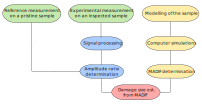
\includegraphics[width=1\linewidth]{Chapter_7/flowchart}
%	%	\end{center}
%	\caption{A flowchart representing the process for damage size estimation.}
%	\label{fig:Flowchart}
%\end{figure}
The \ac{madif} indicates the damage size according to measured damage index \(I\) normalized by the value obtained for the pristine sample \(I^{ref}\).
In the paper, two types of damage index \(I\) are considered: the energy \(I_{eng}\) and the maximum value of the half-width of the first package arrived in the sensor \(I_{amp}\), and these are defined as:
\begin{eqnarray}
	I_{eng}(\Phi_D)=\sum_{t=0}^{T} \left (\Psi_g(t,\Phi_D)\right )^2,\quad I_{eng}^{ref}=\sum_{t=0}^{T} \left (\Psi_g(t,0)\right )^2,\\
	I_{amp}(\Phi_D)=\mathrm{max}\left ( \Psi_g(t,\Phi_D)\right ),\quad I_{amp}^{ref}=\mathrm{max}\left ( \Psi_g(t,0)\right ),
	\label{eq:I_amp}
\end{eqnarray}
where \textit{T} is a period of the signal.
\(\Psi_g(t,\Phi_D)\) is for the damaged case scenario, whereas \(\Psi_g(t,0)\) is for the pristine sample and it is realized in the same way by windowing the full-length signals of the sensor \(\Psi(t)\) with a flattened Gaussian window \emph{g(t)} as follows:
\begin{eqnarray}
	\Psi_g(t)=\Psi(t)g(t)= \Psi(t)\mathrm{exp}\left(-\left(\frac{t-t_0}{0.6005612w_g}\right) ^{12}\right),
	\label{eq:psi_g}
\end{eqnarray}
where \(t_0\) is the center and \(w_g=0.5N_c/f_c\) is a half-width of the window.
Windowing the signals ensures obtaining the signals without any reflections from the boundaries.
The determination of \(\Psi_g\) is pictured in Figure~\ref{fig:window_madif}a.

\begin{figure}[H]
	%	\begin{center}
	\includegraphics[width=1\linewidth]{Chapter_7/window_madif_03}
	%	\end{center}
	\caption{(\textbf{a}) The %MDPI: The hyphen in the picture should be changed to minus sign, e.g., ``-0.5'' to ``$-$0.5'', please change. Please check all like this in all figures. 
		sensor signal \(\Psi(t)\) windowed by a flattened Gaussian window \(g(t)\) and (\textbf{b}) the damage size estimation from the \ac{madif}.}
	\label{fig:window_madif}
\end{figure}
In the time domain, an equivalent numerical signal to the signal registered by the \ac{pzt} acquisition instrument is calculated as an average value of the electrical potential of the electrode surface
\begin{eqnarray}
	\Psi^{n}(t) = \frac{\int_{\Gamma_e}\phi\mathrm{d}\Gamma}{\Gamma_e},
	\label{eq:psi}
\end{eqnarray}
where \(n=1\) and \(n=2\) correspond to the homogenized and presented model, respectively.

The \ac{madif} is achieved by approximating the inverse of the computed damage index that best matches the experimental one.
Finally, the damage size \(\Phi_D\) is obtained from the \ac{madif} curve for measuring the normalized value of \(I/I^{ref}\) as it is presented in Figure~\ref{fig:window_madif}b.